\subsection{Performance of the Filter}
The position Kalman filter is tested in a similar way as the attitude one. The simulations have been performed by applying some inputs to the simulation model of the system. The signals coming out of the model are then extracted and some noise is added to them. The noisy signals are used as the input to the position Kalman filter in order to evaluate its performance. The amount of noise added is the same as that present in the real sensors, the variance values can be seen in \autoref{app:IMUvariances}.\fxnote{write variances used for the kalman filter.}

In \autoref{fig:sim_xn}, the results for the $x_\mathrm{n}$ estimation can be seen.
\begin{figure}[H]
    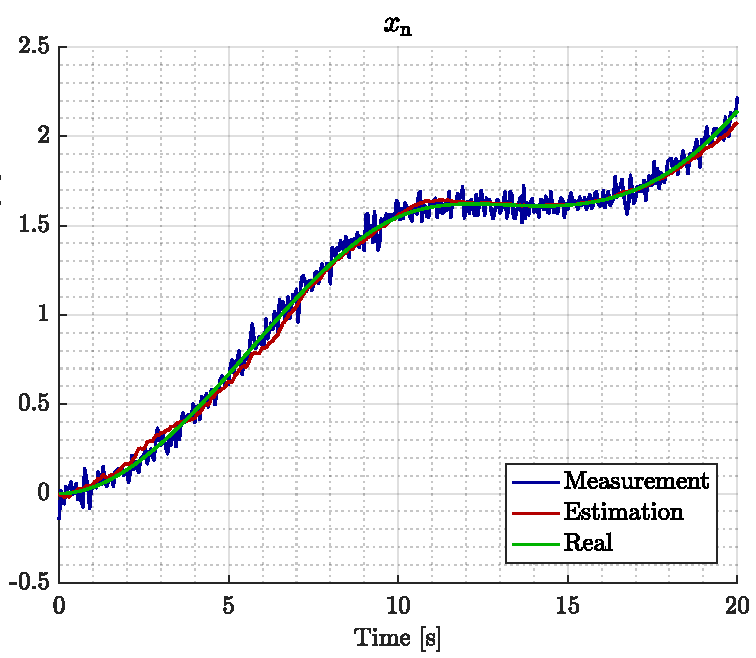
\includegraphics[width=0.5\textwidth]{figures/sim_xn}
    \caption{Measurement, real value and estimation of $x_\mathrm{n}$.}
    \label{fig:sim_xn}
\end{figure}

They show that the filter is able to remove the noise of the measurements and produce an estimation very closed to the real position.

The filter is also tested for the estimation of $\dot{x}_\mathrm{b}$ and $\ddot{x}_\mathrm{b}$, as seen in \autoref{fig:sim_xbdot} and \autoref{fig:sim_xbddot}, respectively.

\begin{figure}[H]
    \captionbox 
    {   
        Result of the estimation of the translational velocity along $x_\mathrm{b}$, compared to the real value in the simulation..
        \label{fig:sim_xbdot}
    }                                                                 
    {                                                                  
        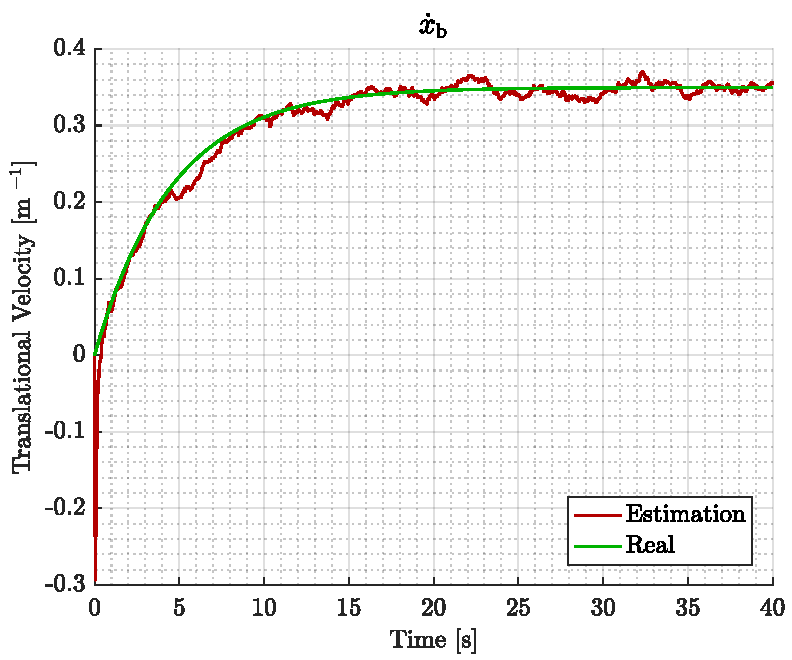
\includegraphics[width=.45\textwidth]{figures/sim_xbdot}         
    }                                                                    
    \hspace{5pt}                                                          
    \captionbox  
    {      
        Estimation of the translational acceleration along $x_\mathrm{b}$, compared to the real value and the measurements.
        \label{fig:sim_xbddot}
    }                                                                          
    {
        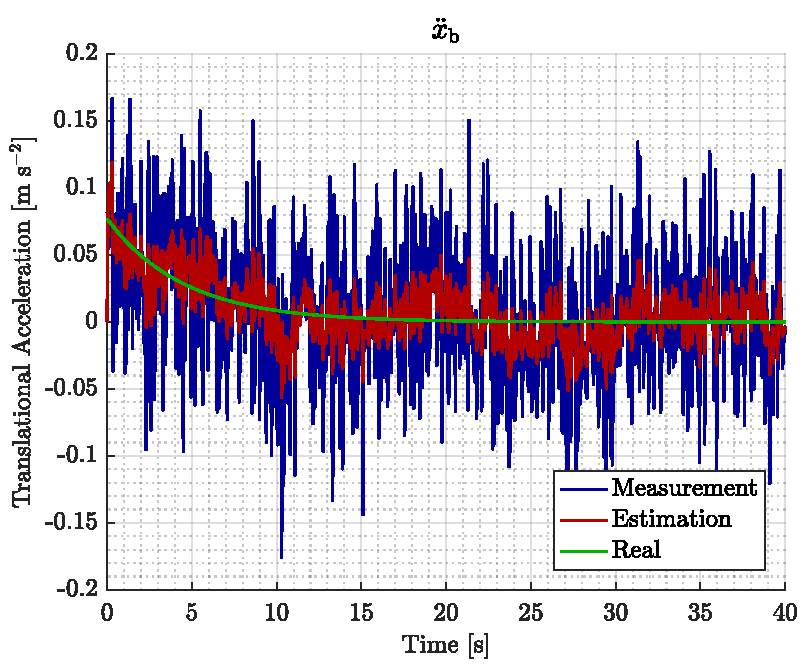
\includegraphics[width=.45\textwidth]{figures/sim_xbddot}
    }
\end{figure}

The estimation of $\ddot{x}_\mathrm{b}$ is able to remove the noise that comes from the measurements, and the filter is as well able to give a close estimation of $\dot{x}_\mathrm{b}$ even though there is no measurement on that variable.